\documentclass[../analysisII_notes.tex]{subfiles}
\begin{document}
\section{Aula 16 - 07 de Maio, 2025}
\subsection{Motivações}
\begin{itemize}
	\item Convergência Uniforme.
\end{itemize}
\subsection{Convergência Uniforme.}
Dada uma sequência de funções \(f_{n}:X\rightarrow \mathbb{R}\), estudamos até o momento o que é a convergência pontual, ou ponto-a-ponto, dela. Hoje, queremos continuar com mais exemplos e definir o que será a convergência uniforme, além de compará-la, ao longo das próximas aulas, com a convergência pontual.

O problema que estudaremos a seguir é sumarizado na pergunta ``para quais pontos no domínio de f existe o limite \(\lim_{n\to \infty}f_{n}(x)\)?'', além de formarmos e caracterizarmos os elementos do conjunto
\[
	\mathfrak{C}\coloneqq \{x\in X: \exists \lim_{n\to \infty}f_{n}\}.
\]

Começamos a buscar nossas respostas por meio de alguns exemplos:
\begin{example}
	A sequência \(f_{n}:\mathbb{R}\rightarrow \mathbb{R}\) dada por \(f_{n}(x)=\cos^{}{(nx)}\), sendo n um número natural, não converge pontualmente para nenhuma função, pois para todo x real, o limite
	\[
		\lim_{n\to \infty}\cos^{}{(nx)}
	\]
	não existe - ele fica oscilando muito, nunca ``parando quieto''. Por exemplo, quando x vale \(\pi \), esse limite seria o limite alternado \((-1)^{n}\), o qual não converge.
\end{example}
\begin{example}
	Seja \(f_{n}:\mathbb{R}\rightarrow \mathbb{R}\) dada por
	\[
		f(x)=\sum\limits_{i=0}^{n}x^{i},\quad n\in \mathbb{N}.
	\]
	Como sabemos,
	\[
		f_{n}(x)=\frac{1-x^{n+1}}{1-x},
	\]
	e podemos usar isso para analisarmos os seguintes casos:
	\begin{align*}
		 & |x|<1 \Rightarrow \lim_{n\to \infty}f_{n}(x)=\frac{1}{1-x}                                                                            \\
		 & |x|>1 \Rightarrow \not\exists \lim_{n\to \infty}f_{n}(x)                                                                              \\
		 & |x|=1 \rightarrow \left\{\begin{array}{ll}
			                            x = 1 \Rightarrow f_{n}(1)=\sum\limits_{i=0}^{n}1=n+1 \overbracket[0pt]{\longrightarrow}^{n\to \infty}\infty \\
			                            x= -1 \Rightarrow f_{n}(-1)=1-1+1-1+1-1+1-\dotsc + (-1)^{n}=0 \text{ ou }1.
		                            \end{array}\right.
	\end{align*}
	A conclusão que tiramos é que o conjunto onde a função converge é
	\[
		\mathfrak{C}=(-1, 1) \quad\&\quad f_{n}\overbracket[0pt]{\longrightarrow}^{p}\frac{1}{1-x}.
	\]
\end{example}
\begin{def*}
	Dizemos que uma função \(f:X\rightarrow \mathbb{R}\) \textbf{converge uniformemente para uma função }\(f:X\rightarrow \mathbb{R}\)\textbf{ em X}, e escrevemos
	\[
		f_{n}\overbracket[0pt]{\rightarrow}^{u}f
	\]
	em X se, para todo \(\varepsilon >0\), existe \(n_{0}\) natural tal que, \textit{para todo} x em X e \(n\geq n_{0}\),
	\[
		|f_{n}(x)-f(x)|<\varepsilon .
	\]
	Em outras palavras, se para todo \(\varepsilon > 0\), existir \(n_{0}\) tal que, se \(n\geq n_{0}\),
	\[
		\sup_{x\in X}|f_{n}(x)-f(x)|<\varepsilon .\quad \square
	\]
\end{def*}
A ideia dessa definição é que, dados \(\varepsilon \) positivo e uma função com domínio X e contradomínio nos reais, a \textit{faixa ao redor de f de raio }\(\varepsilon \) contém todos os gráficos das \(f_{n}\)'s. Com efeito, fixada a faixa
\[
	\mathcal{F}(f;\varepsilon )=\{(x, y)\in \mathbb{R}^{2}:\: x\in X \:\&\:f(x)-\varepsilon <y<f(x)+\varepsilon \},
\]
dizer que \(f_{n}\) converge para f uniformemente no domínio X significa que existe um \(n_{0}\) natural tal que os gráficos das \(f_{n}\)'s estão todos contidos em \(\mathcal{F}(f;\varepsilon )\), pois
\[
	n\geq n_{0},\: x\in X \Rightarrow f(x)-\varepsilon  < f_{n}(x)<f(x)+\varepsilon .
\]

\begin{figure}[H]
	\begin{center}
		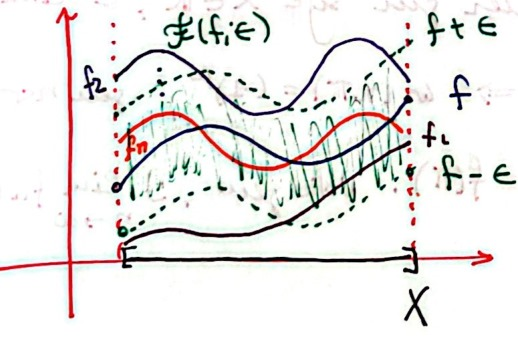
\includegraphics[height=0.5\textheight, width=0.5\textwidth, keepaspectratio]{./Images/epsilon_band_16.png}
	\end{center}
	\caption{visualização da faixa definida na interpretação da convergência uniforme.}
	\label{epsband16}
\end{figure}

\begin{prop*}
	Se \(f_{n}\) converge uniformemente para f em X, então \(f_{n}\) converge para f pontualmente em X.
\end{prop*}
\begin{proof*}
	Com efeito, se \(x_{0}\) for um ponto de X e supusermos que \(f_{n}\) converge uniformemente para f, podemos usar a definição com o supremo para obter a desigualdade
	\[
		|f_{n}(x_{0})-f(x_{0})|\leq \sup_{x\in X}|f_{n}(x)-f(x)|.
	\]
	Portanto, dado \(\varepsilon > 0\), existe \(n_{0}\) natural tal que, se \(n\geq n_{0}\), teremos
	\[
		|f_{n}(x_{0})-f(x_{0})|<\varepsilon ,
	\]
	que é exatamente o mesmo que
	\[
		\lim_{n\to \infty}f_{n}(x_{0})=f(x_{0}) \quad \forall x_{0}\in X. \quad \text{\qedsymbol}
	\]
\end{proof*}

Duas coisas muito úteis que tiramos desse teorema é que, por sua contra positiva, uma função não convergente no sentido pontual também não poderá convergir uniformemente. A outra, por outro lado, garante que ao sabermos que uma função converge pontualmente, podemos testar para a convergência uniforme.
\begin{example}
	A convergência da função
	\[
		f_{n}(x)=\frac{x}{n}\rightarrow0
	\]
	não é uniforme em \(\mathbb{R}\), pois qualquer \(\varepsilon \) positivo resulta numa faixa que não contém o gráfico de nenhuma dS \(f_{n}\)'s, pois, se \(\varepsilon > 0\) for fixo e n for um natural, sempre existirá um número real \(x\) tal que
	\[
		\biggl\vert \frac{x}{n} \biggr\vert \geq \varepsilon ,
	\]
	bastando escolher x tal que \(|x|\geq \varepsilon n\).
	\begin{figure}[H]
		\begin{center}
			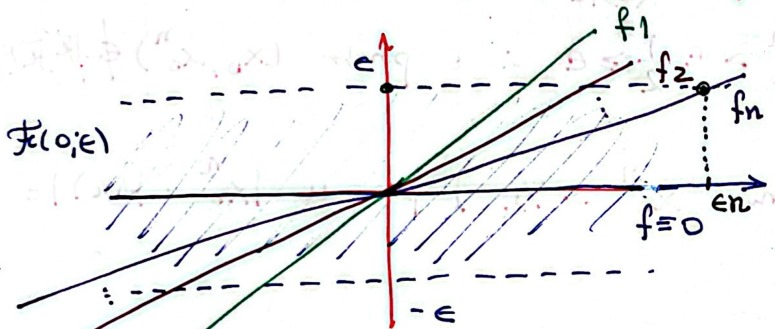
\includegraphics[height=0.5\textheight, width=0.5\textwidth, keepaspectratio]{./Images/converging_uniformly_16.png}
		\end{center}
		\caption{a função \(f_{n}\) do exemplo sempre escapa da faixa \(\varepsilon \), não importa o n.}
	\end{figure}

	Porém, ao restringirmos as funções a um intervalo \([a, b]\) qualquer, então
	\[
		f_{n}\overbracket[0pt]{\longrightarrow}^{u}0
	\]
	em \([a, b]\). Com efeito, escolha \(M>0\) tal que \([a, b]\subseteq [-M, M]\) e note que, para todo \(\varepsilon > 0\), se \(n_{0}\) for maior que a divisão de M por \(\varepsilon ,\) então
	\[
		n\geq n_{0} \Rightarrow \biggl\vert \frac{x}{n} \biggr\vert \leq \frac{M}{n_{0}}<\varepsilon ,
	\]
	ou seja,
	\[
		n\geq n_{0} \Rightarrow \sup_{x\in [-M, M]}|f_{n}(x)-0|<\varepsilon.
	\]

	Disto, concluímos que a convergência é pontual em toda a reta \(\mathbb{R}\) e uniforme em todo compacto da reta
\end{example}

\begin{example}
	Considere, agora, a sequência de funções \(f_{n}:[0, 1]\rightarrow \mathbb{R}\) dada por
	\[
		f_{n}(x)=x^{n},
	\]
	a qual converge pontualmente para
	\[
		x^{n}\overbracket[0pt]{\rightarrow}^{p} f(x)= \left\{\begin{array}{ll}
			0, & \quad x\in [0,1) \\
			1, & \quad x=1.
		\end{array}\right.,
	\]
	mas ela não é uniforme; por exemplo, se \(\varepsilon \) for tomado entre 0 e 0.5, a faixa \(\mathcal{F}(f;\varepsilon )\) não conterá o gráfico de nenhuma das \(f_{n}\)'s e,  para ilustrar isso, podemos tomar um natural n qualquer, tal que, por conta de
	\[
		\lim_{x\to 1^{-}}x^{n}=1,
	\]
	existirá um valor \(x_{0}\) no intervalo \([0, 1)\) com
	\[
		x_{0}^{n}>\frac{1}{2}\geq \varepsilon .
	\]
	Portanto, o ponto \((x_{0}, x_{0}^{n})\) nunca pertencerá à faixa \(\mathcal{F}(f;\varepsilon )\), pois
	\[
		|x_{0}^{n}-f(x_{0})|=x_{0}^{n}>\frac{1}{2}\geq \varepsilon .
	\]
	\begin{figure}[H]
		\begin{center}
			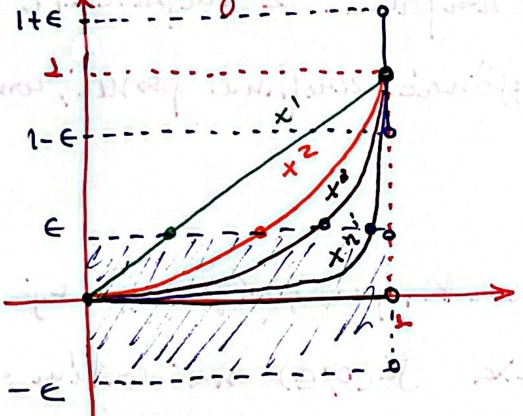
\includegraphics[height=0.5\textheight, width=0.5\textwidth, keepaspectratio]{./Images/xn_16.png}
		\end{center}
		\caption{a partir de certo ponto, os termos da sequência fogem do intervalo que define a faixa.}
	\end{figure}

	Por outro lado, se \(\delta \) for um valor entre 0 e 1, a convergência de \(f_{n}\) para f será uniforme nos compactos \([0, 1-\delta ]\). De fato, note que f é identicamente nula dentro de cada intervalo \([0, 1-\delta ]\) e, além disso, como \(0<1-\delta <1\),
	\[
		0\leq x\leq 1-\delta \Rightarrow 0\leq x^{n}<(1-\delta )^{n}\overbracket[0pt]{\longrightarrow}^{n\to \infty}0,
	\]
	ou seja, para n suficientemente grande,
	\[
		\sup_{0\leq x\leq 1-\delta }|x^{n}-f(x)|=\sup_{0\leq x\leq 1-\delta }|x|^{n}<(1-\delta )^{n}<\varepsilon
	\]
\end{example}

\begin{def*}
	Dizemos que \(f_{n}:X\rightarrow \mathbb{R}\) é uma \textbf{sequência de Cauchy em X} quando, para todo \(\varepsilon \) positivo, existir um natural \(n_{0}\) tal que
	\[
		m, n\geq n_{0} \Rightarrow |f_{m}(x)-f_{n}(x)|<\varepsilon ,\quad \forall x\in X.
	\]
	Equivalentemente,
	\[
		m, n\geq n_{0} \Rightarrow \sup_{x\in X}\{f_{m}(x)-f_{n}(x)\}<\varepsilon .\quad \square
	\]
\end{def*}
\end{document}
